%!TEX root = root.tex

\chapter{Comprehensive discovery of driver genes and mutations in cancer}
\label{chap:ch7}
\chaptermark{Comprehensive driver discovery}

Over the past decade, The Cancer Genome Atlas (TCGA) has coordinated a monumental enterprise of data generation and genomic investigation across 33 cancer types, and numerous notable findings have emerged from this project (\url{https://cancergenome.nih.gov/publications}). The individual TCGA projects also motivated the development of many bioinformatic algorithms oriented toward discovery, characterization, and prioritization of cellular processes driving cancer based on pathways \cite{RN180}, genes \cite{RN49}, or individual variations \cite{RN181}. However, despite this remarkable progress, algorithms do not entirely agree on certain candidate cancer driver genes and mutations, necessitating continued expert curation to filter likely false positive findings. Moreover, previous PanCancer analyses \cite{RN96} have been limited to fewer cancer types and have largely avoided nominating rare driver mutations. 

\section{Mutational data set}
Mutation calls were produced by the Multi-Center Mutation Calling in Multiple Cancers (MC3) working group by harmonizing results of 7 algorithms \cite{RN167}. To reduce the false positive rate for driver gene discovery I implemented three strategies addressing known issues affecting driver detection and data quality (see Mutation calling quality control). The driver detection dataset ultimately consisted of 9,079 samples having 1,457,702 total mutations, where the number of mutations per sample was widely distributed across cancer types and was consistent with previous publications \cite{RN12, RN13, RN96}.

\subsection{Mutation calling quality control}
A publicly available MAF file (\url{https://synapse.org/MC3}) was recently compiled by the MC3 Working Group and is annotated with filter flags to highlight potential artifacts or discrepancies. This dataset represents the most uniform attempt to systematically provide mutation calls for TCGA tumors. The MC3 effort provided consensus calls from 7 software packages \cite{RN167}. Flagged artifacts include: non-exonic regions, whole-genome amplified (WGA) samples, exclusion lists, blood/tumor derived pairs, strand-bias, contamination estimations, oxo-guanine artifacts, low normal read depth, polymorphisms common in EXAC \cite{RN168}, mutations present in a panel of normal samples, non-preferred tumor normal pairs, and mutations outside the regions of interest for any caller. If a mutation was not assigned any flag and was called by 2 or more variant calling software packages, it received a 'PASS' identifier. I restricted our analysis to PASS calls with the exception of samples from OV and LAML, which were some of the earliest sequenced by TCGA. Preparations for these samples utilized whole genome amplified (WGA) DNA, an important factor in that the WGA process can induce artefactual mutations. Of the 412 OV and 141 LAML samples present in our data 347 (84\%) and 141 (100\%), respectively, had variants derived from WGA DNA. In order to maintain sample sizes and uniformity in mutation calling, I did not filter mutations containing only 'wga' filter tags from these two cancer types. I recognize multiple limitations of this mutation call set including the lack of structural variants and copy number alterations, as well as variability in sequencing depth and tumor purity. The above limitations may lead to variability in mutation detection; however, the MC3 dataset reflects the state-of-the-art in consensus mutation detection.

I also excluded highly mutated samples. These hypermutators were defined as samples with a mutation count exceeding Tukey's outlier condition, i.e. greater than 1.5 times the interquartile range above the third quartile in their respective cancer types (3Q + 1.5*IQR). Designation as a hypermutator also required the number of mutations in a sample to exceed 1000, a heuristic that limited the number of discarded samples in low mutation rate cancer types. LUAD, SKCM, and UCEC had hypermutator thresholds greater than 1000 mutations (1047, 2122, and 2545 respectively). I also excluded samples that were flagged by the analysis-working group based on pathology, but allowed "RNA degradation" samples to remain, as this factor is not particularly relevant for most driver prediction tools based on mutations. The final driver-discovery dataset consisted of 9,079 samples having a total of 791,637 missense mutations, 323,884 silent mutations, 96,196 3'UTR mutations, 57,900 nonsense mutations, 42,251 intronic mutations, 42,251 Frame shift deletions, 34,266 5' UTR, 21,804 splice site mutations, 19,856 RNA mutations, 11,305 frame shift insertions, 7,622 3' flanking mutations, 6,419 5' flanking mutations, 6,144 in-frame deletions, 1,362 translation start site mutations, 964 nonstop mutations, and 632 in-frame insertions.

\section{Driver gene discovery approach}
Using multiple tools can overcome numerous technical issues that confound individual statistical analyses to find driver genes, such as heterogeneous mutation rate across the genome \cite{RN13}, inflated significance for long genes \cite{RN169}, and false positive calls in cancers with high mutation rates \cite{RN70}. In the first phase, 8 different tools comprising algorithms based on mutation frequency (MuSiC2 \cite{RN43} and MutSig2CV \cite{RN14}), features (20/20+ \cite{RN70}, CompositeDriver(in preparation) and OncodriveFML \cite{RN86}), clustering (OncodriveCLUST \cite{RN54}), and externally defined regions (e-Driver \cite{RN153} and ActiveDriver \cite{RN98}) were used (\autoref{fig:driver_gene_approach}A). Each tool reported gene or mutation level scores and/or p-values along with a brief description of recommended cutoff thresholds or filters.

\begin{figure}
  \centering
  \makeatletter
  \let\@currsize\normalsize
  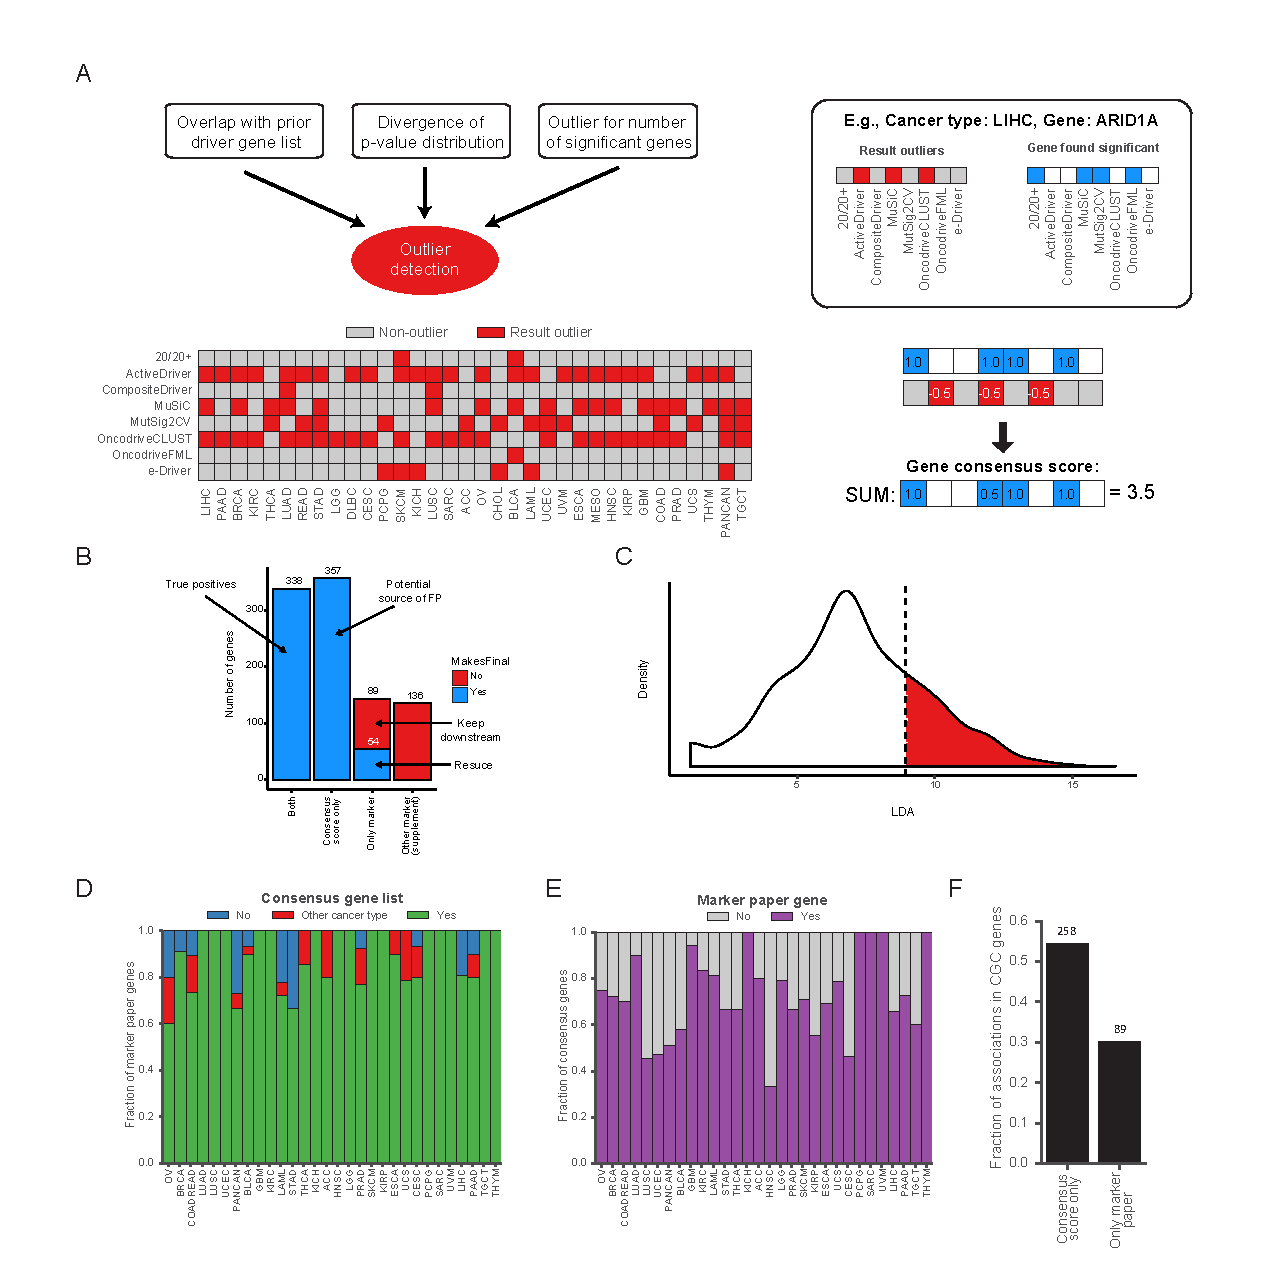
\includegraphics[width=\linewidth]{figures/chapter7/driver_gene_approach.pdf}
  \caption[Consensus Gene scores and SMG filtering.]{Consensus Gene scores and SMG filtering. (A) Left, outlier detection was performed on a per analysis and method basis. Outliers were marked (red) based on the quasi-majority of three criteria: (1) low concordance with known cancer genes from Vogelstein et al (lower than median); (2) high divergence of p-value distribution from theoretical expectation (higher than median); and (3) abnormally high number of significant genes (>1.5x the interquartile range above the third quartile). The first two criteria were assessed based on the other tools within a single analysis, while the third criterion was assessed based on the same tool's results over all the individual cancer types (excluding the PanCancer analysis). Right, example calculation of the gene consensus score for ARID1A in the cancer type LIHC. A result from an outlier is down weighted, receiving a weight of 0.5 instead of 1.0. The gene consensus score is the sum of weights for tools finding that gene as significant. (B) Overlap of consensus gene list with prior TCGA marker papers. (C) Likely false positives were detected with a high Linear Discriminant Analysis (LDA) score threshold representing 90\% sensitivity for keeping associations found in Cancer Gene Census genes. LDA was trained to distinguish common false positives in exome sequencing from previous TCGA PanCancer marker papers. The LDA threshold was only applied to the potential source of false positive genes. (D) Fraction of marker paper genes highlighted in the main text that were also found in our consensus gene list. (E) Fraction of our consensus gene list found in previous TCGA marker papers.  (F) Fraction of associations found in the Cancer Gene Census (CGC) that were either found only in the consensus gene list or TCGA marker paper. }
  \label{fig:driver_gene_approach}
\end{figure}

\subsection{Consensus methodology}
I identified a preliminary total of 2,101 potential drivers by taking the union of genes predicted by the eight driver-gene discovery tools.  As illustrated in \autoref{fig:driver_gene_approach}A, the increased number of false positive genes is likely due to any individual tool's capability to maintain sound statistical properties that handle a complex set of factors such as tumor heterogeneity, increased mutation rates, and variable sample sizes. I refined this list by calculating, for each gene predicted in each cancer type, a consensus score that compensated for outlier results and correlation among tools (\autoref{fig:driver_gene_approach}). The consensus score was defined as a weighted sum of the number of tools that predicted the gene to be a driver in each cancer type (see \autoref{sec:weighting}). I required a minimum of two tools to agree, where both could not be outliers (score$\geq$1.5). Although it is difficult to distinguish the overall performance improvement on a small number of held out CGC genes (\autoref{fig:gene_characteristics}A), the weighting strategy did have higher specificity (p=4.3e-8, McNemar test), which is preferable given concerns of false positives. Regardless, the consensus score performance on identifying CGC genes (\autoref{fig:gene_characteristics}A) support previous reports that merging the results from different algorithms improve cancer driver discovery \cite{RN96}. 

\begin{figure}
  \centering
  \makeatletter
  \let\@currsize\normalsize
  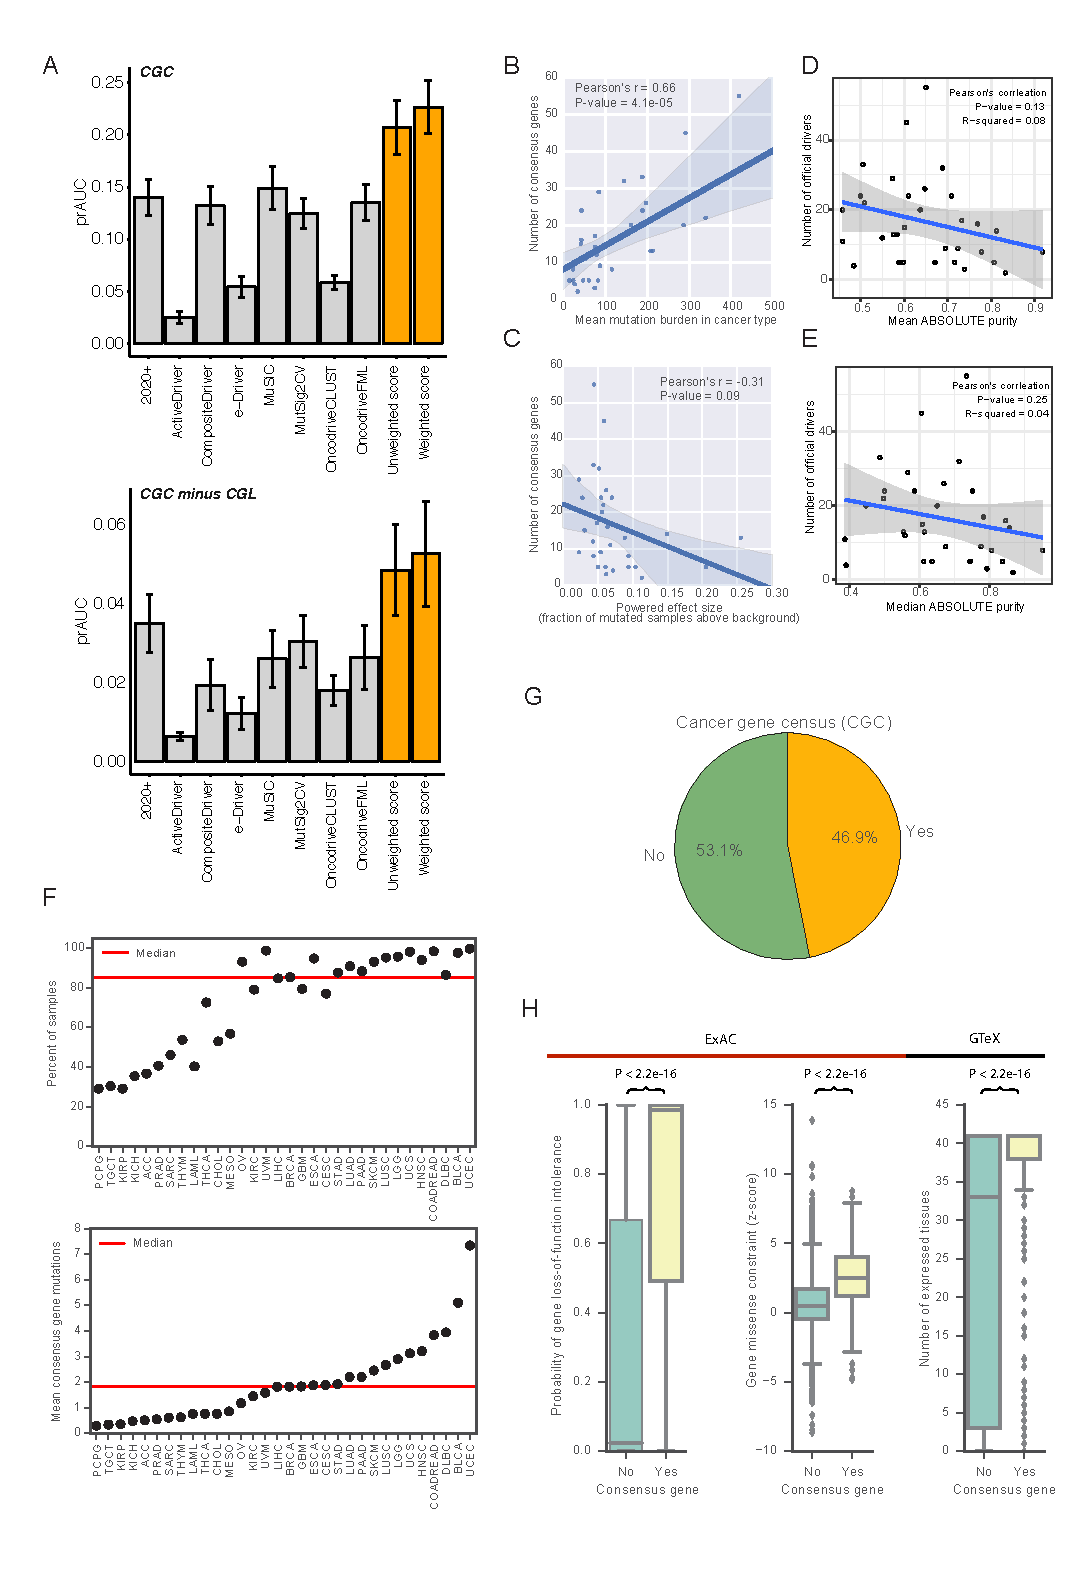
\includegraphics[width=\linewidth]{figures/chapter7/analysis_of_cancer_driver_genes.pdf}
  \caption[Characteristics of consensus genes.]{Characteristics of consensus genes. (A) Predictive power of each individual driver gene detection method (in gray) and of the weighted and weighted scores (in orange). The predictive power was measured as prAUC, using all the genes in the Cancer Gene Census and a set that additionally excludes Cancer Genome Landscape genes used in outlier detection. Error bars, calculated by bootstrapping, indicate one standard deviation. (B) The number of consensus genes in each cancer type positively correlated with the average mutation burden. Shaded area indicates 95\% bootstrapped confidence interval. (C) Given the variability in powered effect size (fraction of mutated samples above background with 90\% power) in this study, there is a negative but not significant correlation with the number of consensus genes in each cancer type. COAD and READ were excluded because analysis was performed separately, but the final consensus genes were merged. (D) Pearson correlation between the number driver genes identified and median purity was calculated and plotted. (E) Pearson correlation between the number driver genes identified and mean purity was calculated and plotted. Summary statistics for p-value and r-squared value are reported in the top right corner of panels D and E. (F) Percent of samples containing a non-silent mutation stratified by cancer type. The red line indicates the median across cancer types (left) and average number of non-silent mutations in consensus genes per sample (right). (G) A pie chart showing the percent of consensus genes which are found in the Cancer Gene Census with annotations for small somatic mutations (missense, splice site, indel, and nonsense) (H) Consensus genes showed a higher probability for loss-of-function intolerance and missense mutation constraint of germline mutations based on ExAC, and were expressed (RPKM>1) in a wider number of tissues from GTeX (version 6). Given the high correlation of gene expression in the 11 brain regions assessed from GTEx, we took the median of multiple brain tissues, as done in Lek et al., 2016.}
  \label{fig:gene_characteristics}
\end{figure}

To maximize the coverage of our analysis and ensure the accuracy of our final list, previous findings were reviewed in 31 individual cancer types and PanCancer-12 from TCGA. For cancer types not yet having a TCGA publication, the relevant analysis working groups were consulted (LIHC, TGCT, UVM, SARC, PAAD, and THYM). I included in our final consensus list all those genes that were previously described as drivers by experts in the cancer-specific analysis of TCGA datasets and were also identified by at least one of the eight algorithms, even if they did not meet our consensus score threshold ($\geq$1.5)(\autoref{fig:gene_discovery}A). This resulted in an additional 54 gene-cancer pairs, such as ATR, CHEK2, IDH2, and ERCC2 in the PanCancer dataset and FOXA1 in BLCA, HRAS in SKCM, and MET in LUAD (\autoref{ref:driver_gene_approach}B-F). The majority of this effort resulted in linking cancer genes identified by our strategy to additional cancer types based on previous literature (32/54).  

\begin{figure}
  \centering
  \makeatletter
  \let\@currsize\normalsize
  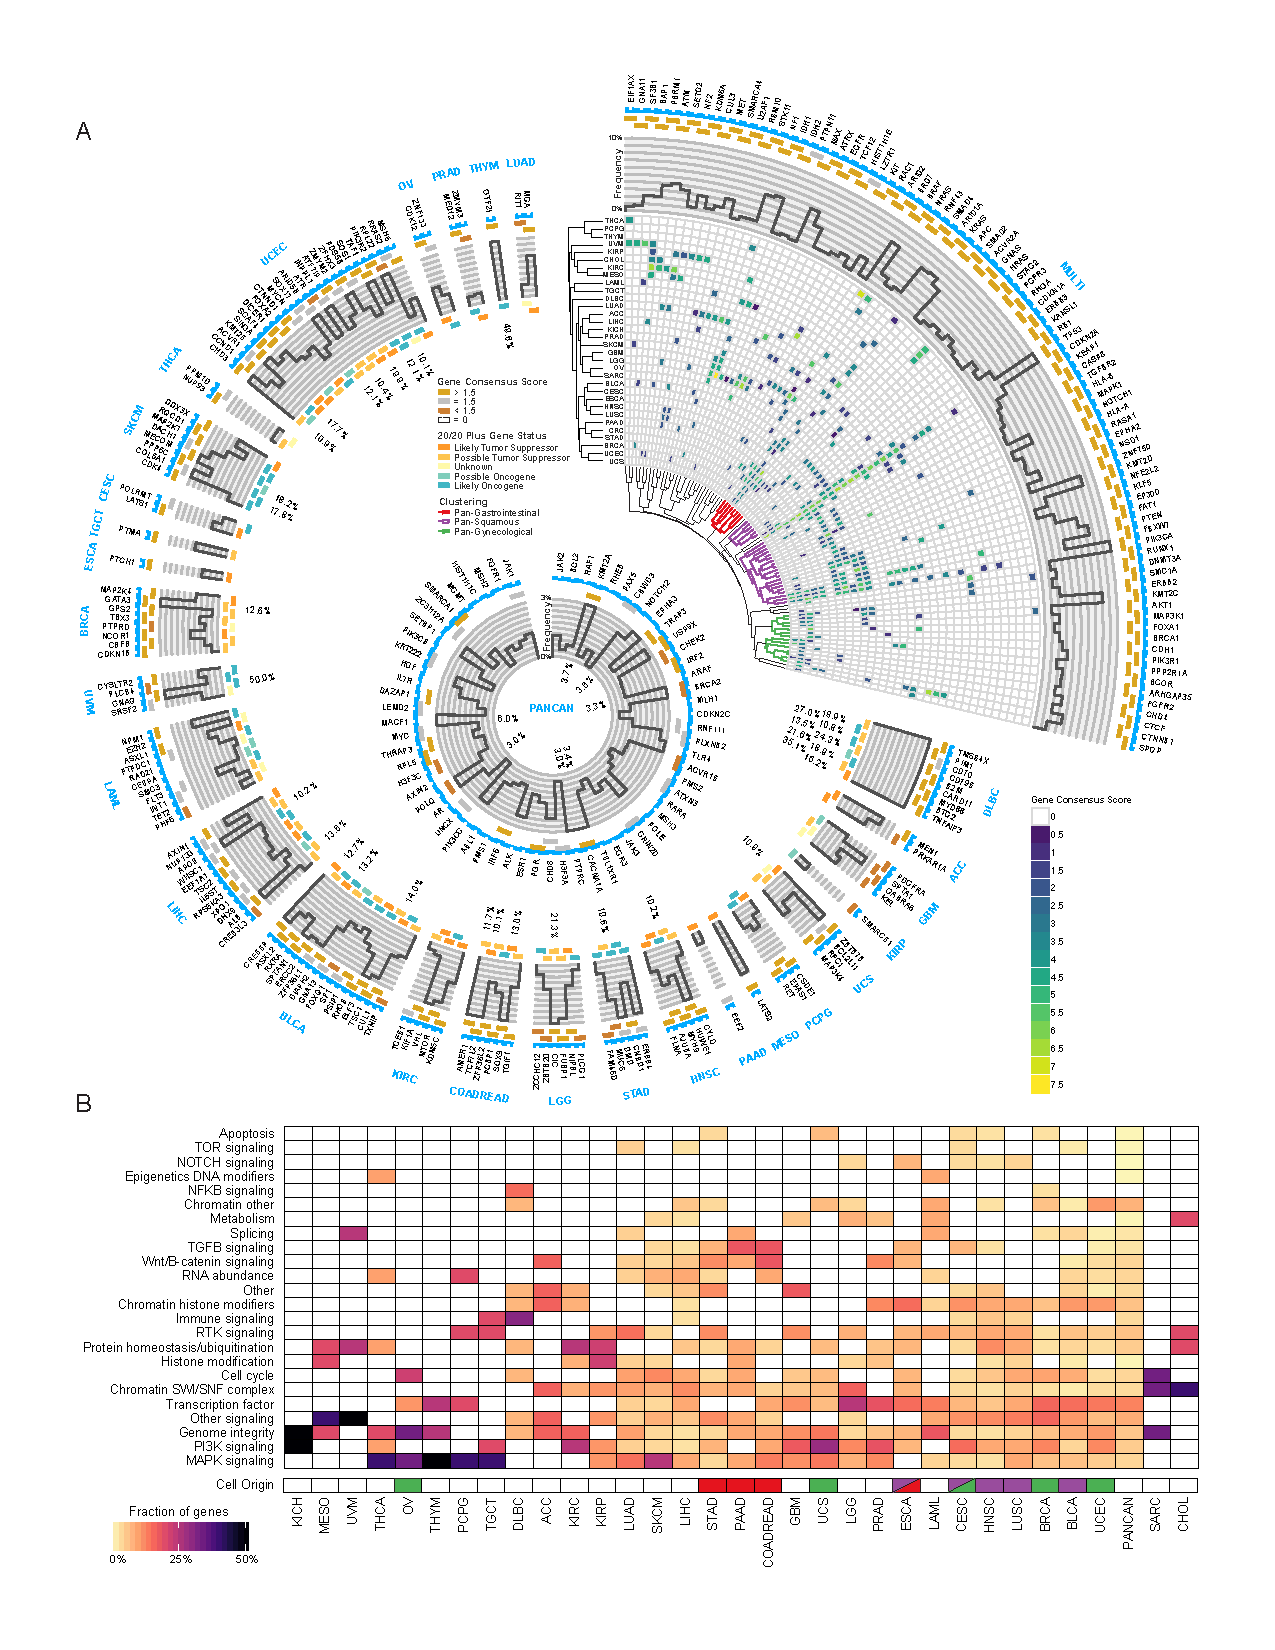
\includegraphics[width=\linewidth]{figures/chapter7/cancer_driver_genes.pdf}
  \caption[Cancer driver gene discovery]{Cancer driver gene discovery: (A) Circos \cite{RN182} plot displays 299 cancer genes. Each sector indicates a unique cancer type (text in blue) with predicted drivers unique to that cancer type listed (gene name in black). Only tissues with at least one unique driver gene are shown. The top right sector shows all genes found significant in multiple cancer types. Next, a categorical score of gold, silver, or bronze is assigned to each gene based on the highest consensus score. If a gene was not scored and required rescue then the field is empty. The next ring illustrates the mutation frequency of a gene in our dataset. For the top right wedge, the PanCancer frequency is used, while cancer-type-specific frequencies are used in the remaining sectors. Where frequencies exceed the y-axis limit of 10\%, the innermost label indicates the frequency. The final ring uses a 5-point scale from orange to teal to represent each gene from likely tumor suppressor to likely oncogene, respectively, by the 20/20+ algorithm. Finally, in the top right slice we show hierarchical clustering of the gene consensus scores for genes that were found in more than one cancer type (note: CRC refers to the COADREAD cancer type). Additionally, significant gene clusters (permutation test) identified Pan-Gastrointestinal (red), Pan-Squamous (purple), and Pan-Gynecological tissues (green). The middle ring illustrates all genes that were only found using PanCancer results, or were otherwise rescued. (B) Heatmap showing clustering of different cancer types by pathway / biological process affected by associated consensus driver genes. Cell of origin for pan-gynecological, pan-gastrointestinal, and pan-squamous are colored as above.}
  \label{fig:gene_discovery}
\end{figure}

To limit false positives in the expanded list, linear discriminant analysis was applied (\autoref{ref:driver_gene_approach}C). 45 genes were identified and removed from the consensus as they are likely false positives. These included CACNA1E in PanCancer, COL11A1 in LUAD, DST in GBM, and TTN in SKCM. The consensus list from the above systematic approach consisted of 258 unique genes. The average number of non-silent mutations per sample in our consensus gene list varied substantially by cancer type ranging from <1 in 12 cancer types (ACC, CHOL, KICH, KIRP, LAML, MESO, PCPG, PRAD, SARC, TGCT, THCA, and THYM) to 7.3 in UCEC. A median of 85\% of tumors harbored non-silent mutations in consensus genes across cancer types (\autoref{fig:gene_characteristics}F). 

Given the limitations of a systematic approach, 41 genes were manually rescued. In the rescue attempt, I started with a list of genes identified from previous TCGA marker papers but not found from our systematic approach. Genes were rescued with supportive evidence from the following sources: hypermutator phenotype related genes (since we excluded hypermutated samples in our systematic discovery; 6 genes), established cancer genes from LAML because of low quality variant calling originating from liquid tumor contamination of the normal samples (6 genes), genes supported by omic network tools (DriverNet and OncoIMPACT; 25 genes), and a gene supported by all three approaches from the driver mutation discovery (1 gene). Addition of genes to the final list was subjected to expert manual curation (3 genes). 

The final consensus gene list consisted of 299 unique genes across 33 cancer types and the PanCancer dataset (\autoref{fig:gene_discovery}A). The list captures most previously described driver genes for the majority of cancer types. I overlapped the cancer driver genes obtained from the consensus approach without manual curation with those from 5 independent studies in 4 cancer types (BRCA, PRAD, PAAD, and LIHC) of which one is whole-genome sequencing. The consensus approach always had a greater inter-study overlap, with an average increase of 26\% over only using a single tool, either MuSiC2 or MutSig2CV \cite{RN57, RN176, RN175, RN172, RN173, RN174}. Among the 299 genes, 59 novel genes were not previously identified in 6 previous PanCancer publications \cite{RN57, RN14, RN178, RN25, RN96, RN177, RN1} or the cancer gene census list (\url{http://cancer.sanger.ac.uk/census/})\cite{RN97}.

\subsection{Weighting strategy}
\label{sec:weighting}
Tools predicting cancer genes were weighted according to their performance in each cancer type, receiving half the weight if a result was deemed an outlier, thereby obligating additional tool agreement. Specifically, I examined quality metrics across tools and within the same tool, which allowed us to identify outlier results. I marked outliers based on the quasi-majority of three criteria: low concordance with known cancer genes, high divergence of p-value distribution from theoretical expectation, and abnormally high number of significant genes. The first criterion evaluated the fraction overlap of significant genes with a previously manually curated set of driver genes from \cite{RN25} compared with the median across all tools. The second criterion examined whether the divergence of observed p-values from those theoretically expected by the Mean Log Fold Change (MLFC) \cite{RN70} was greater than the median of all tools, which may indicate a tool's statistical assumptions may not be well satisfied. The third criterion examined whether a tool's prediction for particular cancer types appeared as an outlier in terms of the number of significant genes compared against all of the results for that tool (Tukey's outlier criterion: number significant $>$ 3Q + 1.5*IQR). I calculated a gene consensus score by summing the tools that declared the gene as being significant, with a weight of 1 for non-outlier results and 0.5 for outlier results.

\section{The landscape of cancer driver genes}



